\documentclass[tikz,border=10pt]{standalone}
% calc is needed for the ($(E)+(dx,dy)$) label offset
\usetikzlibrary{calc}
\begin{document}
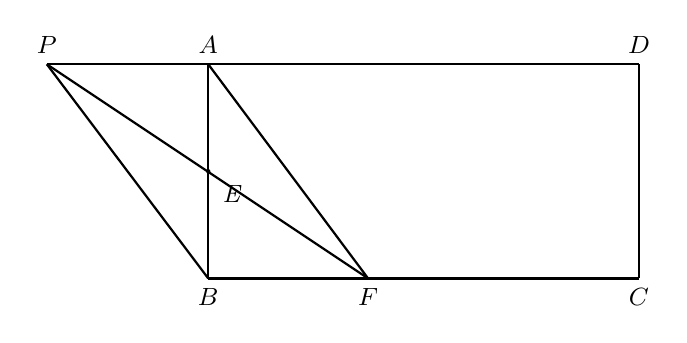
\begin{tikzpicture}[line join=round, line width=0.8pt,
  lbl/.style={font=\fontsize{9}{10.8}\selectfont}]
  % Named coordinates: s = 0.011561 units/px, centre (384,184), y flipped
  \coordinate (P) at (-3.90,  1.36);
  \coordinate (A) at (-1.85,  1.36);
  \coordinate (D) at ( 3.62,  1.36);
  \coordinate (C) at ( 3.62, -1.36);
  \coordinate (B) at (-1.85, -1.36);
  \coordinate (F) at ( 0.18, -1.36);
  % Intersection of PF with AB (E)
  \coordinate (E) at (-1.85, 0);

  % Top segment P-D (passes through A)
  \draw (P) -- (D);
  % Bottom segment B-C (passes through F)
  \draw (B) -- (C);
  % Vertical edges
  \draw (A) -- (B);
  \draw (D) -- (C);
  % Diagonals
  \draw (P) -- (B);
  \draw (A) -- (F);
  \draw (P) -- (F);

  % Small dot at the crossing
  \fill (E) circle (0.8pt);

  % Labels outside the figure
  \node[above, lbl] at (P) {$P$};
  \node[above, lbl] at (A) {$A$};
  \node[above, lbl] at (D) {$D$};
  \node[below, lbl] at (C) {$C$};
  \node[below, lbl] at (B) {$B$};
  \node[below, lbl] at (F) {$F$};
  % Label E just lower-right of the crossing
  \node[anchor=north west, lbl] at ($(E)+(0.05,-0.05)$) {$\mathit{E}$};
\end{tikzpicture}
\end{document}